\section{Rough Work Plan}

The thesis project will, organizationally, be split up into somewhat sprint-like chunks (agile methodology).
Each such \textbf{iteration} will have a duration of \textbf{approx. 4 weeks} and a concrete topic to work on.
At the end of an iteration the results will be reviewed and based on the outcome here the topic for the next one determined. Depending on requirements/circumstances it can also be decided that a respective iteration takes some more or some less time (that is, \textbf{+/- 2 weeks}).
Additionally, an iteration will have some more detailed topic/goal description if respectively applicable.

The whole project shall be finished \textbf{at latest by the end of 2013}.

Though, \textbf{optimistic intent} is to be done by \textbf{summer 2013} already.

The topic of the first iteration is: \textit{``Create Master's Thesis Proposal''}.

It's fluently followed by the 2nd iteration: \textit{``Literature Research \& State of the Art Report''}.

After that, initial actual UI design and implementation of basics of the app should begin.

All in all, there will be around \textbf{8 to 10 iterations} --
consisting of research, analysis, design, implementation, evaluation, and documentation (potentially overlapping and conjoined/intertwined).

Figure~\ref{fig:gantt} shows some Gantt chart diagram visualizing a \textbf{draft project plan}. Provisionally \textit{``Refine...''}-titled iterations can be seen to be generally optional or possibly included within previous iterations, respectively.

\begin{sidewaysfigure}[tb]
  \centering
  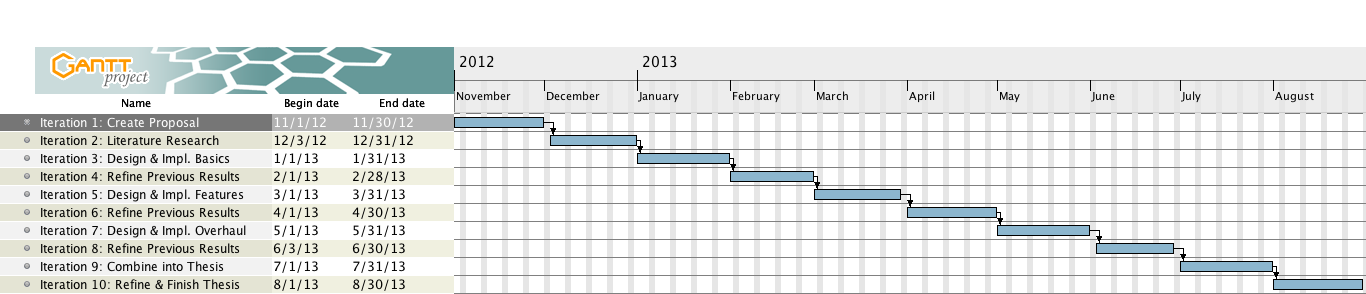
\includegraphics[width=1.0\textwidth]{figures/gantt-draft-project-plan}
  \caption{Draft Gantt chart diagram project plan}
  \label{fig:gantt}
\end{sidewaysfigure}


\section{Preliminary Thesis Structure}

\textbf{N.B.: }this is all subject to change while actually progressing with the thesis project.

\begin{itemize}
  \item Introduction
  	\begin{itemize}
  		\item motivation
  		\item problem statement (which problem should be solved?)
  		\item aim of the work
  		\item methodological approach
  		\item structure of the work
  	\end{itemize}
  \item State of the art / analysis of existing approaches
  	\begin{itemize}
  		\item literature studies
  		\item analysis
  		\item comparison and summary of existing approaches
  	\end{itemize}
  \item Methodology
  	\begin{itemize}
  		\item used concepts
  		\item methods and/or models
  		\item languages
  		\item design methods
  		\item data models
  		\item analysis methods
  		\item formalisms
  	\end{itemize}
  \item Design and implementation of the suggested solution
  \item Critical reflection
  	\begin{itemize}
  		\item comparison with related work
  		\item discussion of open issues
  	\end{itemize}
  \item Summary and future work
  \item ...
\end{itemize}
